\documentclass[t]{beamer}

\mode<presentation> {
\usetheme{CambridgeUS}
}
\usepackage[utf8]{inputenc}
\usepackage[spanish]{babel}
\usepackage{amsmath}
\usepackage{graphicx} 
\usepackage{booktabs} 
\setbeamertemplate{bibliography item}{\insertbiblabel}
\numberwithin{equation}{section}
\usepackage{amsthm}
\newtheorem{definicion}{Definición}
\newtheorem{teorem}{Teorema}


\title[Estrellas de Planck]{Estudio de Estrellas de Planck}

\author[Alejandro Hernández A.]{Alejandro Hernández A. \\ {\ \\ \footnotesize Asesor: Pedro Bargueño.} } 
\institute[Uniandes]  
{\normalsize
Universidad de los Andes, Bogotá, Colombia \\ 
}
\date{Mayo 24, 2016} 

\begin{document}

\begin{frame}
\titlepage 
\end{frame}

\begin{frame}
%[allowframebreaks]
\frametitle{Contenidos} 
\tableofcontents 
\end{frame}

\section{Introducción y motivación}

\begin{frame}{Introducción}
\vspace{\fill}
\begin{itemize}
\item Soluciones estáticas y esféricamente simétricas de las ecuaciones de campo de Einstein (Agujeros negros).
\vspace*{\fill}
%Decir lo de los horizontes de eventos

\item Problemas de las singularidades en el espaciotiempo $\leftrightarrow$ Fallas de la relatividad general.
\vspace{\fill}

\item Agujeros negros regulares.
\end{itemize}
\end{frame}

\begin{frame}{Motivación}
\vspace{\fill}
\begin{itemize}
\item Obtener un conocimiento más profundo de la relatividad general.
\vspace*{\fill}

\item Conocer algunas limitaciones y fallas de dicha teoría.
\vspace*{\fill}

\item Entender la regularización de agujeros negros y los conceptos físicos detrás de este proceso.
\vspace*{\fill}

\item Conocer un poco acerca de teoría cuántica de campos efectiva en relatividad general.
\vspace*{\fill}

%En la medida de lo posible
\end{itemize}
\vspace{\fill}
\end{frame}


\section{\label{preliminaries section} Preliminares}


\subsection{Condiciones de energía}

%Ojo con las implicaciones
\begin{frame}{Condiciones de energía}
\vspace{\fill}
Las condiciones de energía son \cite{carroll,hawking}

\begin{itemize}
\item \textbf{NEC:} $\rho \geq 0$
\vspace*{\fill}
\item \textbf{WEC:} $\rho \geq 0$,  $\rho + p_{i} \geq 0$ para $i \in \{1,2,3\}$.
\vspace*{\fill}
\item \textbf{DEC:} $\rho \geq 0$,  $\rho + p_{i} \geq 0$, $\rho \geq |p_{i}|$ para $i \in \{1,2,3\}$.
\vspace*{\fill}
\item \textbf{SEC:} $\rho + p_{i} \geq 0$ y $\rho + 3p_{i} \geq 0$.
\end{itemize}

%Relaciones DEC -> WEC -> NEC, SEC ->	NEC, SEC does not implies WEC

Para el estudio de agujeros negros regulares, la única condición de energía que nos interesa es la WEC.
\vspace{\fill}
\end{frame}

\subsection{Procedimiento General}

\begin{frame}{Procedimiento general}
Forma general del elemento de línea esféricamente simétrico y estático:

\begin{equation}
\label{general static spherical}
ds^2 = -f(r)dt^2 + \frac{1}{f(r)}dr^2 + r^2d\Omega^2,
\end{equation}

\begin{equation}
\label{general f}
f(r) = 1 - \frac{2m(r)}{r}.
\end{equation}

En términos de $m(r)$ la WEC se expresa como \cite{vanegas-weak}

\begin{equation}
\label{mass wec ineq}
\begin{aligned}
\frac{1}{r^2}\frac{dm(r)}{dr} &\geq 0,\\
\frac{2}{r}\frac{dm(r)}{dr} &\geq \frac{d^2m(r)}{dr^2}.
\end{aligned}
\end{equation}

\end{frame}

\section{\label{previous metrics section} Métricas relevantes}


\subsection{\label{bardeen section} Métrica de Bardeen}
\begin{frame}{Métrica de Bardeen}
\vspace{\fill}
La métrica de Bardeen está dada por \cite{bardeen}
\small
\begin{equation}
\label{bardeen metric}
ds^2 = -\left( 1 - \frac{2mr^2}{(r^2 + g^2)^{3/2}} \right)dt^2 + \left( 1 - \frac{2mr^2}{(r^2 + g^2)^{3/2}} \right)^{-1}dr^2 + r^2d\Omega^2,
\end{equation}

\normalsize
\begin{equation}
f_{bardeen}(r) \underset{r \to 0}{\sim} 1 - \frac{2mr^2}{g^3} + \mathcal{O}(r^4),
\end{equation}

\begin{equation}
f_{bardeen}(r) \underset{r \to \infty}{\sim} 1 - \frac{2m}{r} + \frac{3mg^2}{r^3} + \mathcal{O}\left( \frac{1}{r^5} \right).
\end{equation}
\vspace{\fill}
\end{frame}

\begin{frame}{Métrica de Bardeen}
Los invariantes de curvatura de esta métrica están dados por

\begin{equation}
\label{bardeen scalars}
\begin{gathered}
R = \frac{6 g^2 m \left(4 g^2-r^2\right)}{\left(g^2+r^2\right)^{7/2}},\\
R_{\mu \nu}R^{\mu \nu} = \frac{18 g^4 m^2 \left(8 g^4-4 g^2 r^2+13 r^4\right)}{\left(g^2+r^2\right)^7},\\
R_{\mu \nu \sigma \rho}R^{\mu \nu \sigma \rho} = \frac{12 m^2 \left(8 g^8-4 g^6 r^2+47 g^4 r^4-12 g^2 r^6+4 r^8\right)}{\left(g^2+r^2\right)^7}.
\end{gathered}
\end{equation}
\end{frame}

\begin{frame}{Métrica de Bardeen}
La condición de energía débil se satisface automáticamente puesto que al considerar la función de masa
\begin{equation}
m(r) = \frac{mr^3}{(r^2 + g^2)^{3/2}},
\end{equation}

se tiene que
\begin{align}
\begin{aligned}
\frac{1}{r^2}\frac{dm(r)}{dr} &= \frac{6 m g^2}{\left(g^2+r^2\right)^{5/2}},\\
\frac{2}{r}\frac{dm(r)}{dr} &= \frac{12 m g^2 r}{\left(g^2+r^2\right)^{5/2}},\\
\frac{d^2m(r)}{dr^2} &= \frac{6 m \left(2 g^4 r-3 g^2 r^3\right)}{\left(g^2+r^2\right)^{7/2}}.
\end{aligned}
\end{align}
\end{frame}

\begin{frame}{Métrica de Bardeen}
Para la interpretación física de la métrica de Bardeen, se requiere acoplar RG con electrodinámica no-lineal \cite{ayon-beato2000}

\begin{equation}
\mathcal{S} = \int dv \left( \frac{1}{16 \pi}R - \frac{1}{4 \pi}\mathcal{L}(F) \right),
\end{equation}

\begin{equation}
\label{nonlinear bardeen}
\mathcal{L}(F) = \frac{3}{2sg^2}\left( \frac{\sqrt{2g^2F}}{1 + \sqrt{2g^2F}} \right)^{5/2},\ s = \frac{|g|}{2m}
\end{equation}

Con el ansatz $F_{\mu \nu} = 2 \delta^{\theta}_{\ \lbrack\mu} \delta^{\varphi}_{\ \nu\rbrack} B(r, \theta)
$,

\begin{equation*}
\frac{1}{4 \pi} \int_{S^{\infty}}\mathbf{F} = \frac{g}{4 \pi} \int_{0}^{\pi}\int_{0}^{2\pi}\sin (\theta) d\theta d\varphi = g
\end{equation*}

$ \leadsto g$ corresponde a la carga de monopolo autogravitante.
\end{frame}

\begin{frame}{Métrica de Bardeen}
Para la interpretación del carácter regular de la métrica de Bardeen

\begin{figure}[h!]
	\centering
	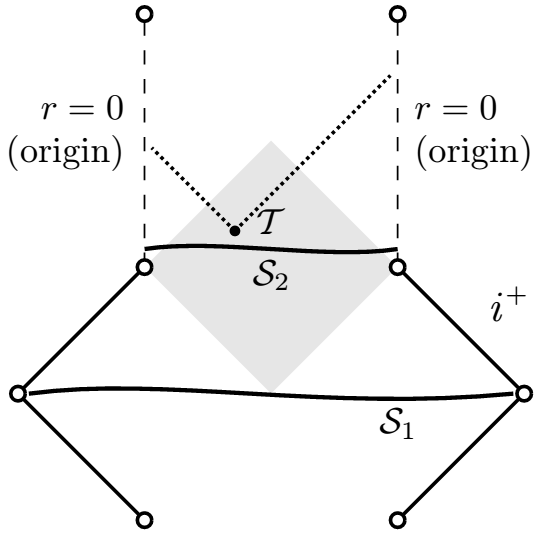
\includegraphics[width=0.35\textwidth]{bardeenDiagram}
	\caption{Estructura global de una porción del agujero negro de Bardeen. Imagen tomada de \cite{borde1994}.}
	\label{fig: bardeen diagram}
\end{figure}
\end{frame}

\begin{frame}{Métrica de Bardeen}
\vspace{\fill}
\begin{teorem}[Borde, 1996]
	\label{borde reg thm}
	Suponga que una espaciotiempo $\mathcal{M}$ satisface que
	
	\begin{enumerate}[i]
		\item contiene una superficie eventualmente futuramente atrapada $\mathcal{T}$,
		
		\item obedece la condición de convergencia nula,
		
		\item el conjunto de geodésicas nulas futuras es completo,
		
		\item su futuro causal es simple, con $E^{+}(X) \neq \emptyset,\ \forall X \subset \mathcal{M} \text{\ acronal}$.
	\end{enumerate}
	
	Entonces hay una sección espacial compacta en el futuro de $\mathcal{T}$.
\end{teorem}
\vspace{\fill}
\end{frame}

\begin{frame}{Métrica de Bardeen}
\begin{teorem}[Penrose, 1965]
\label{penrose sing thm}
Si un espaciotiempo satisface que

\begin{enumerate}[i]
\item contiene una hipersuperficie de Cauchy $\Sigma$ no-compacta y conexa,

\item contiene una superficie cerrada futuramente atrapada (future-trapped surface),

\item cumple con la condición de convergencia nula $R_{\mu \nu}u^{\mu}u^{\nu} \geq 0$ para cualquier vector nulo $u^{\mu}$ (o equivalentemente, cumple la NEC),
\end{enumerate}

entonces dicho espacio tiempo posee geodésicas incompletas de tipo nulo futuro.
\end{teorem}

Un \textbf{horizonte de Cauchy} básicamente es una superficie que separa dos regiones del espacio: una que contiene geodésicas cerradas tipo espacio y otra que contiene curvas cerradas tipo tiempo.
\end{frame}

\subsection{Métrica de Vaidya}

\begin{frame}{Métrica de Vaidya}
En la métrica de Schwarzschild, considerar

\begin{equation}
dt = du + \frac{dr}{(1 - 2m/r)},
\end{equation}

y al generalizar $m = m(u)$, se obtiene

\begin{equation}
\label{schw-tortoise}
ds^2 = - \left(1- \frac{2m(u)}{r}\right)du^2 - 2dudr + r^2d\Omega^2.
\end{equation}

%El SET asociado es
%
%\begin{equation}
%T_{uu} = -(m'/4 \pi r^2),\ m' = dm(u)/du
%\end{equation}
%
%corresponde a radiación saliente.

Diferencia crucial con Schwarzschild: $r = 2m(u)$ deja de ser un horizonte de eventos y se convierte en un horizonte aparente.

\begin{definicion}[Horizonte aparente]
Un horizonte aparente es una hipersuperficie que separa las regiones que poseen superficies atrapadas de las regiones que no contienen este tipo de superficies.
\end{definicion}

\end{frame}


\section{\label{planck stars section} Métrica de Hayward}


\subsection{Métrica de Hayward estática}

\begin{frame}{Métrica de Hayward estática}
La métrica de Hayward está dada por

\begin{equation}
\label{hayward metric}
ds^2 = -\left( 1 - \frac{2mr^2}{r^3 + 2ml^2} \right) dt^2 + \left( 1 - \frac{2mr^2}{r^3 + 2ml^2} \right)^{-1} dr^2 + r^2d\Omega ^2,
\end{equation}

\begin{equation}
f_{hayward}(r) \underset{r \to 0}{\sim} 1 - \frac{r^2}{l^2} + \mathcal{O}(r^5),
\end{equation}

\begin{equation}
f_{hayward}(r) \underset{r \to \infty}{\sim} 1 - \frac{2m}{r} + \frac{4l^2m^2}{r^4} + \mathcal{O}(r^{-5}),
\end{equation}

¿Interpretación física del parámetro $l$?
\
\\
\
\\
¿Cómo aplica el teorema de Borde en este caso?
\end{frame}

\begin{frame}{Métrica de Hayward estática}
\vspace{\fill}
Los invariantes de curvatura de esta métrica son

\begin{equation}
\label{hayward scalars}
\begin{gathered}
R = \frac{24 l^2 m^2 \left(4 l^2 m-r^3\right)}{\left(2 l^2 m+r^3\right)^3},\\
R_{\mu \nu}R^{\mu \nu} = \frac{288 m^4 \left(8 l^8 m^2-4 l^6 m r^3+5 l^4 r^6\right)}{\left(2 l^2 m+r^3\right)^6},\\
R_{\mu \nu \sigma \rho}R^{\mu \nu \sigma \rho} = \frac{48 m^2 \left(32 l^8 m^4-16 l^6 m^3 r^3+72 l^4 m^2 r^6-8 l^2 m r^9+r^{12}\right)}{\left(2 l^2 m+r^3\right)^6},
\end{gathered}
\end{equation}
\end{frame}

\begin{frame}{Métrica de hayward estática}
\vspace*{\fill}
Nuevamente se satisface la condición de energía débil puesto que dada la función de masa
\begin{equation}
\label{hayward mass}
m(r) =  \frac{mr^3}{r^3 + 2ml^2}.
\end{equation}

tenemos que
\begin{equation}
\begin{aligned}
\frac{1}{r^2}\frac{dm(r)}{dr} &= \frac{12 l^2 m^2}{\left(2 l^2 m+r^3\right)^2},\\
\frac{2}{r}\frac{dm(r)}{dr} &= \frac{24 l^2 m^2 r}{\left(2 l^2 m+r^3\right)^2},\\
\frac{d^2m(r)}{dr^2} &= \frac{48 m^2 \left(l^4 m r-l^2 r^4\right)}{\left(2 l^2 m+r^3\right)^3}.
\end{aligned}
\end{equation}
\end{frame}


\subsection{Métrica de Hayward dinámica}

\begin{frame}{Métrica de Hayard dinámica}
\vspace*{\fill}
Al considerar 
\begin{equation}
dt = du + \frac{dr}{(1 - 2m(r)/r)}.
\end{equation}

y generalizar $m = m(u)$ tenemos que 
\begin{equation}
\label{hayward-tortoise}
ds^2 = -\left( 1 - \frac{2m(u)r^2}{r^3 + 2m(v)l^2} \right) du^2 - 2dudr + r^2d\Omega ^2,
\end{equation}

\end{frame}


\subsection{Métrica de Hayward modificada}

\begin{frame}{Métrica de Hayward modificada}
\vspace*{\fill}
Las métricas de las estrellas de Planck deberían incluir \cite{lorenzo}

\begin{itemize}
\item La corrección de loop quantum gravity al potencial Newtoniano, dada por

\begin{equation}
\label{newF}
\Phi (r) = -\frac{m}{r} \left( 1 + \beta \frac{l_{p}^2}{r^2} \right) + \mathcal{O}(r^{-4}).
\end{equation}

\item Dilatación de tiempo finita entre $r$ = 0 y $r \to \infty$.
\end{itemize}

\end{frame}

\begin{frame}{Métrica de Hayward Modificada}
Dado que 
\begin{equation}
\label{newton - metric}
g_{00} = - (1 + 2\phi),
\end{equation}

para incluir las correcciones previamente mencionadas se da la métrica
\begin{equation}
\label{reg-schF}
ds^2 = -G(r)F(r) dt^2 + \frac{1}{F(r)} dr^2 + r^2d\Omega^2,
\end{equation}

donde

\begin{equation}
\label{mod-hay-f}
F(r) = 1 - \frac{2mr^2}{r^3 + 2ml^2},
\end{equation}

y la función $G(r)$ se explica a continuación.

\end{frame}

\begin{frame}{Métrica de Hayward Modificada}
Las condiciones físicas que se le exigen a $G(r)$ son
\begin{itemize}
\item Preservar el comportamiento de Schwarzschild para $r \to \infty$.
\item Incluir la corrección cuántica del potencial newtoniano \eqref{newF}.
\item Permitir dilataciones de tiempo finitas entre $r \to 0$ y $r \to \infty$.
\end{itemize}

La forma más general de satisfacer las condiciones anteriormente impuestas es considerar $G(r)$ dada por

\begin{equation}
\label{mod-hay-g}
G(r) = 1 - \frac{\beta M \alpha}{\alpha r^3 + \beta M},
\end{equation}

donde $\alpha$ está dado por

\begin{equation}
-g_{00}(r = 0) = 1 - \alpha,\ 0 \leq \alpha < 1.
\end{equation}
\end{frame}


\section{\label{conclusions} Conclusiones}

\begin{frame}{Conclusiones}
\begin{itemize}
\item La teoría de la relatividad general clásica presenta fallas potencialmente debidas a la no cosideración de la teoría cuántica.
\vspace*{\fill}
\item El proceso de regularización de agujeros negros puede ser esclarecido mediante la inclusión de la teoría cuántica en gravedad.
\vspace{\fill}
\item Las estrellas de Planck son una alternativa de regularización de agujeros negros, que plantea una nueva instancia el la vida de un agujero negro.
\vspace*{\fill}
\item Las estrellas de Planck pueden alcanzar una densidad del orden de la densidad de Planck a escalas de longitud mucho mayores que la longitud de Planck.
\end{itemize}
\end{frame}


\begin{frame}
\frametitle{Trabajo Futuro}
\vspace*{\fill}
\begin{itemize}
\item Entender profundamente el teorema de Borde y sus múltiples aplicaciones en este trabajo.

\vspace*{\fill}
\item Entender el carácter regular de la métrica de Bardeen en términos del teorema de Borde.

\vspace*{\fill}
\item Entender la derivación de las correcciones de teoría cuántica de campos efectiva del potencial Newtoniano.

\vspace*{\fill}
\item Entender la solución de la paradoja de la pérdida de información en agujeros negros \cite{rovelliquantum}.
\end{itemize}
\vspace{\fill}
\end{frame}

\section{Referencias}
\begin{frame}[t, allowframebreaks]{Referencias}
\footnotesize
\bibliographystyle{unsrt}
\bibliography{Biblio}
\end{frame}
 

\begin{frame}
\Huge{
\
\\
\vspace*{\fill}
\centerline{
¡Gracias por su atención!}
}
\vspace*{\fill}
\end{frame}


\end{document} 